\section{Method}

Our method works on top of existing $EM$ agglomeration algorithms such as \textit{NeuroProof} or \textit{GALA} (CITE BOTH). First we use a 3D U-net to generate voxel affinities predicting the probability that two voxels belong to the same neuron. The \textit{zwatershed} algorithms takes these affinities and generates an oversegmentation of the neurons (CITE). \textit{NeuroProof} agglomerates these supervoxels by training a multi-level random forest classifier. We use a low threshold for neuroproof to generate an oversegmentation. 

In order to use graph-based optimization strategies we need to generate nodes $N$ and edges $E$ for the graph $G$. 

\subsection{Graph Creation}

\subsubsection{Node Generation}

The simplest method of generating nodes is to create one node for every unique segment label in a volume. However, there are many small segments that remain after NeuroProof that only introduce noise when moving to a higher level of abstraction. For now, we decide to remove these segments from consideration and focus on the only the large segments that have expansive spans through the volume. Every segment with fewer than $20,000$ voxels is pruned from the set of considered nodes. Figure \ref{fig:skeletonization} shows two typical segments that each have one corresponding node in the graph $G$. 

\subsubsection{Edge Generation}

\begin{figure}[t]
	\centering
	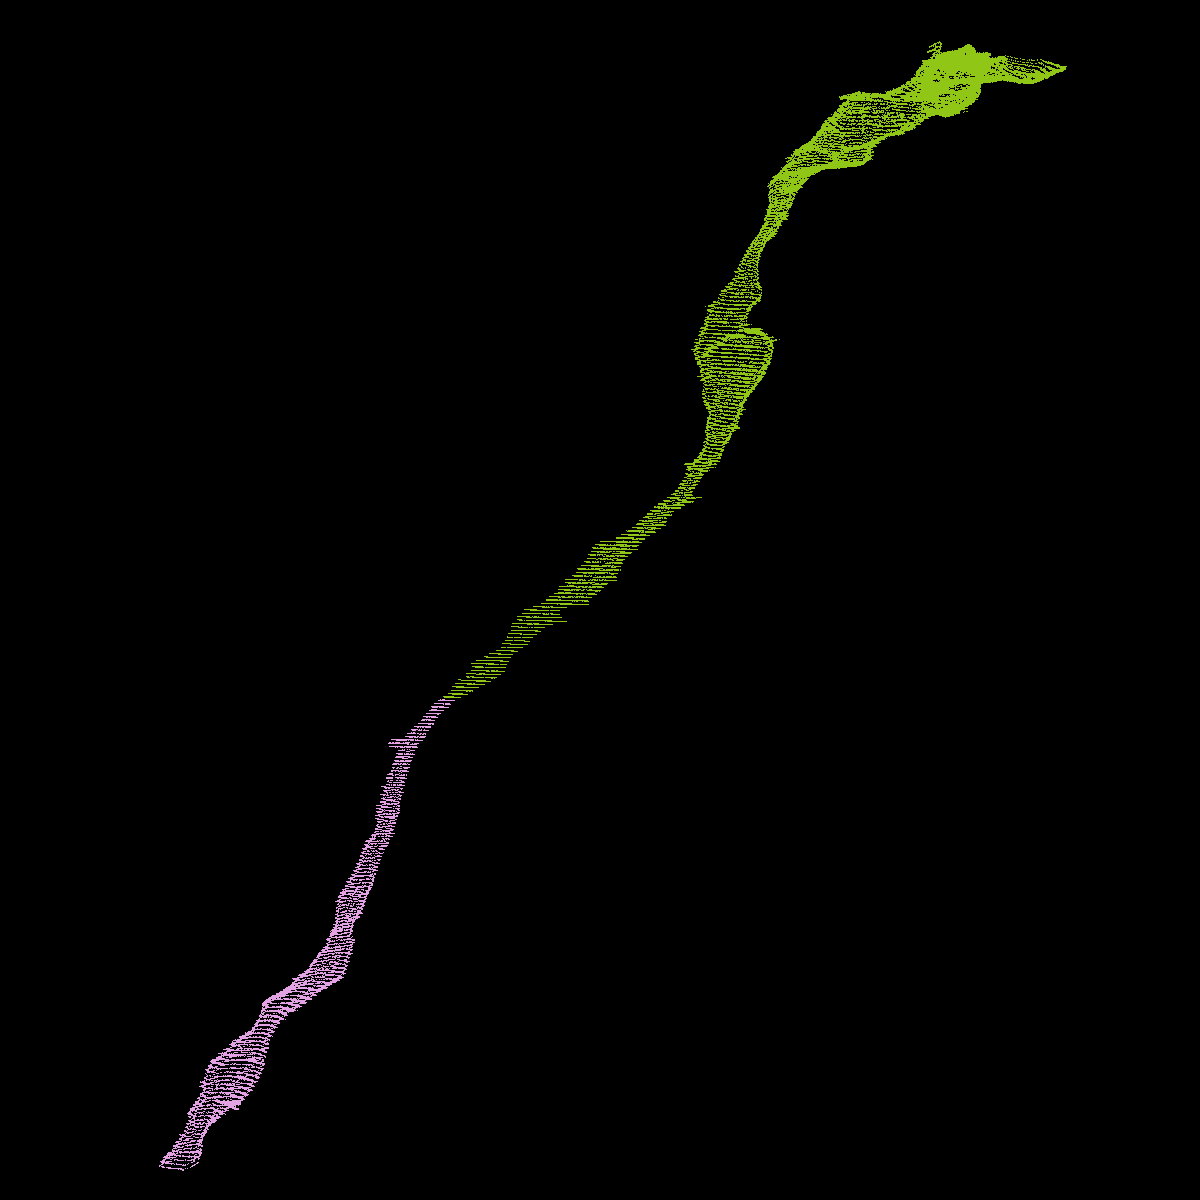
\includegraphics[width=0.42\linewidth]{./figures/merge_candidate1.png}
	\hspace{0.085\linewidth}
	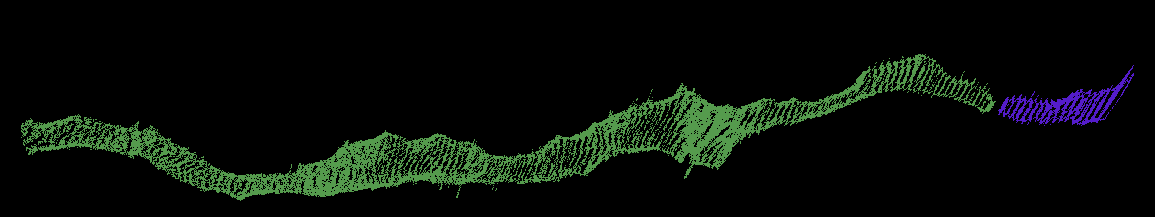
\includegraphics[width=0.42\linewidth]{./figures/merge_candidate2.png}
	\caption{Two erroneously split segments that should merge together. Most segments that we want to merge have the same general structure.}
	\label{fig:merge_candidates}
\end{figure}


The na\"ive edge generation approach is just to simply consider all nodes whose segmentations have a neighboring voxel. Current agglomeration approaches such as NeuroProof or GALA use this criteria for deciding which segments could potentially form one neuron. However, this produces too many edges in our graph, many of which are easily prunable. In fact, many of the segments that we need to merge have very similar structures. Consider Figure \ref{fig:merge_candidates} which shows two erroneously split segments. In both instances the segments around the break follow the same general shape. The segment is more-or-less tubular in the close vicinity with an abrupt break at the end of segment where the next segment begins. The following algorithm identifies these locations without introducing as much ``noise" as using the na\"ive strategy. 

We begin by generating skeletons for every segment. The intuition behind this decision is that a skeleton is a simplified representation of the overarching shape of a segment. Figure \ref{fig:skeletonization} shows two example segments and their corresponding skeletons in white. These skeletons were generated using the Tree-structure Extraction Algorithm for Accurate and Robust Skeletons (TEASER) \cite{sato2000teasar} which has been used in connectomics research previously \cite{zhao2014automatic}. The skeleton consists of a series of \textit{joints} with edges between neighboring joints. Joints that have only one neighbor are also called \textit{endpoints}. Joints that are within $50$ voxels of each other are pruned to reduce unnecessary branching. 

After skeletonization, we proceed to identify locations between segments that we should consider for merging. The algorithm proceeds in two passes. In the first pass we iterate over every endpoint, $e$, in all of the skeletons and create a set $S_e$ where the set includes every segment that has a single voxel with $t_{low}$nm from the endpoint. This first pass often includes too many negative merge candidates leaving a very unbalanced set of merge/split candidates (FIX THIS). Therefore, in our second pass we iterate over all of the endpoints and their corresponding sets. We find the closest endpoint for a given segment $s \in S_e$ to the endpoint $e$. If the closest endpoint is less than $t_{high}$nm from the original endpoint $e$, we add an edge in the graph between these two segments. We also store the midpoint between the closest endpoint and the original endpoint $e$, which will be useful in the following section. Algorithm \ref{alg:generate-edges} provides pseudocode for this edge generation algorithm. The results in this paper follow from $t_{low} = 240nm$ and $t_{high} = 600nm$. 

\begin{figure}[t]
	\centering
	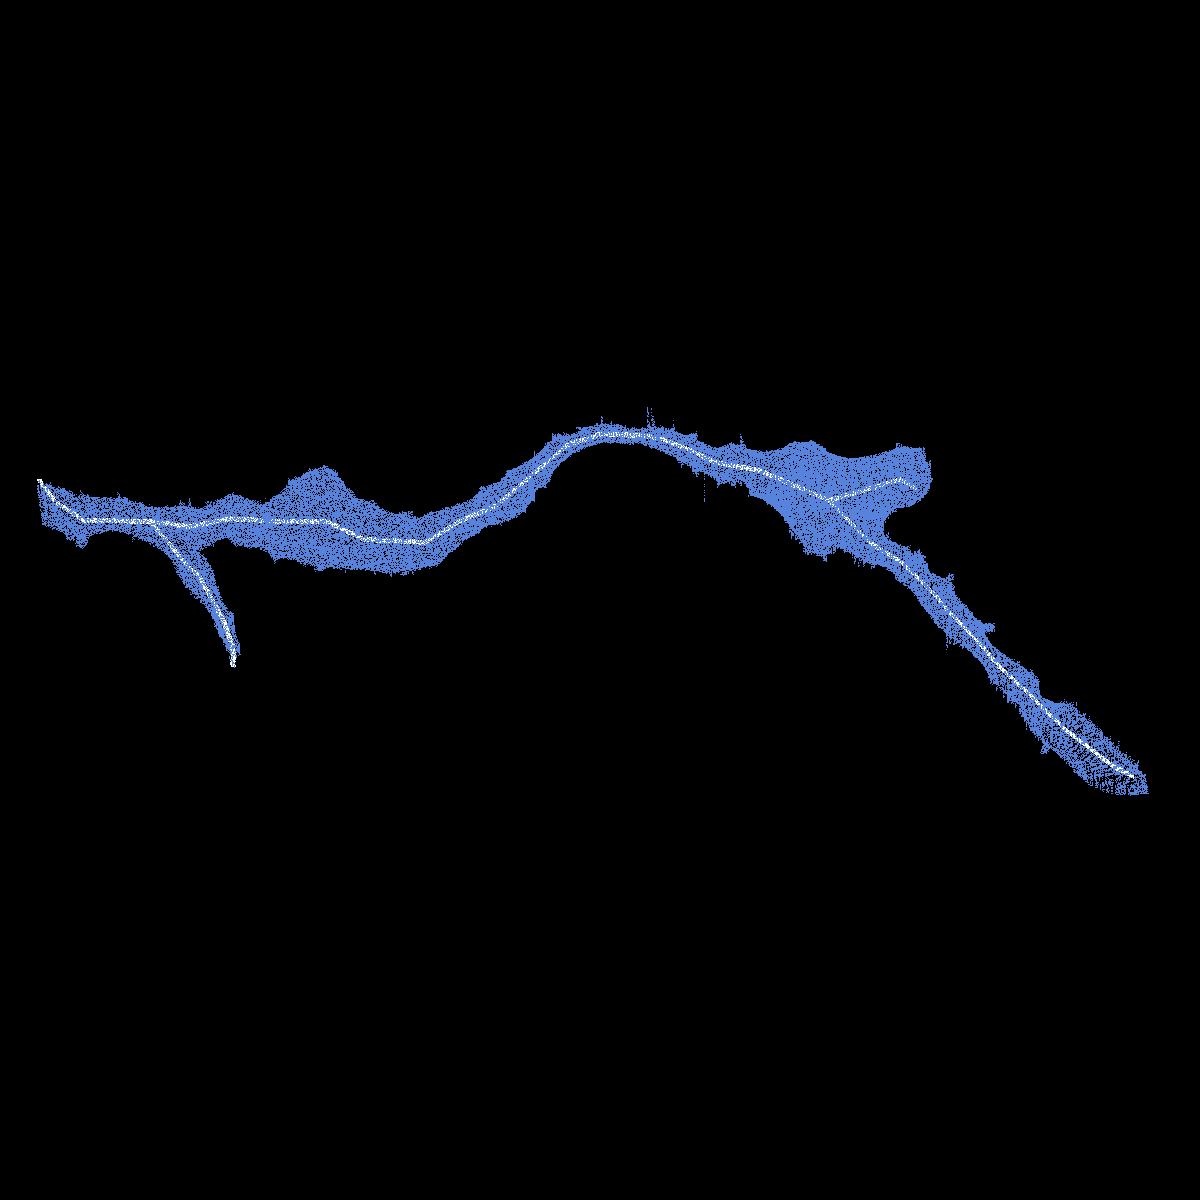
\includegraphics[width=0.42\linewidth]{./figures/skeleton1.png}
	\hspace{0.085\linewidth}
	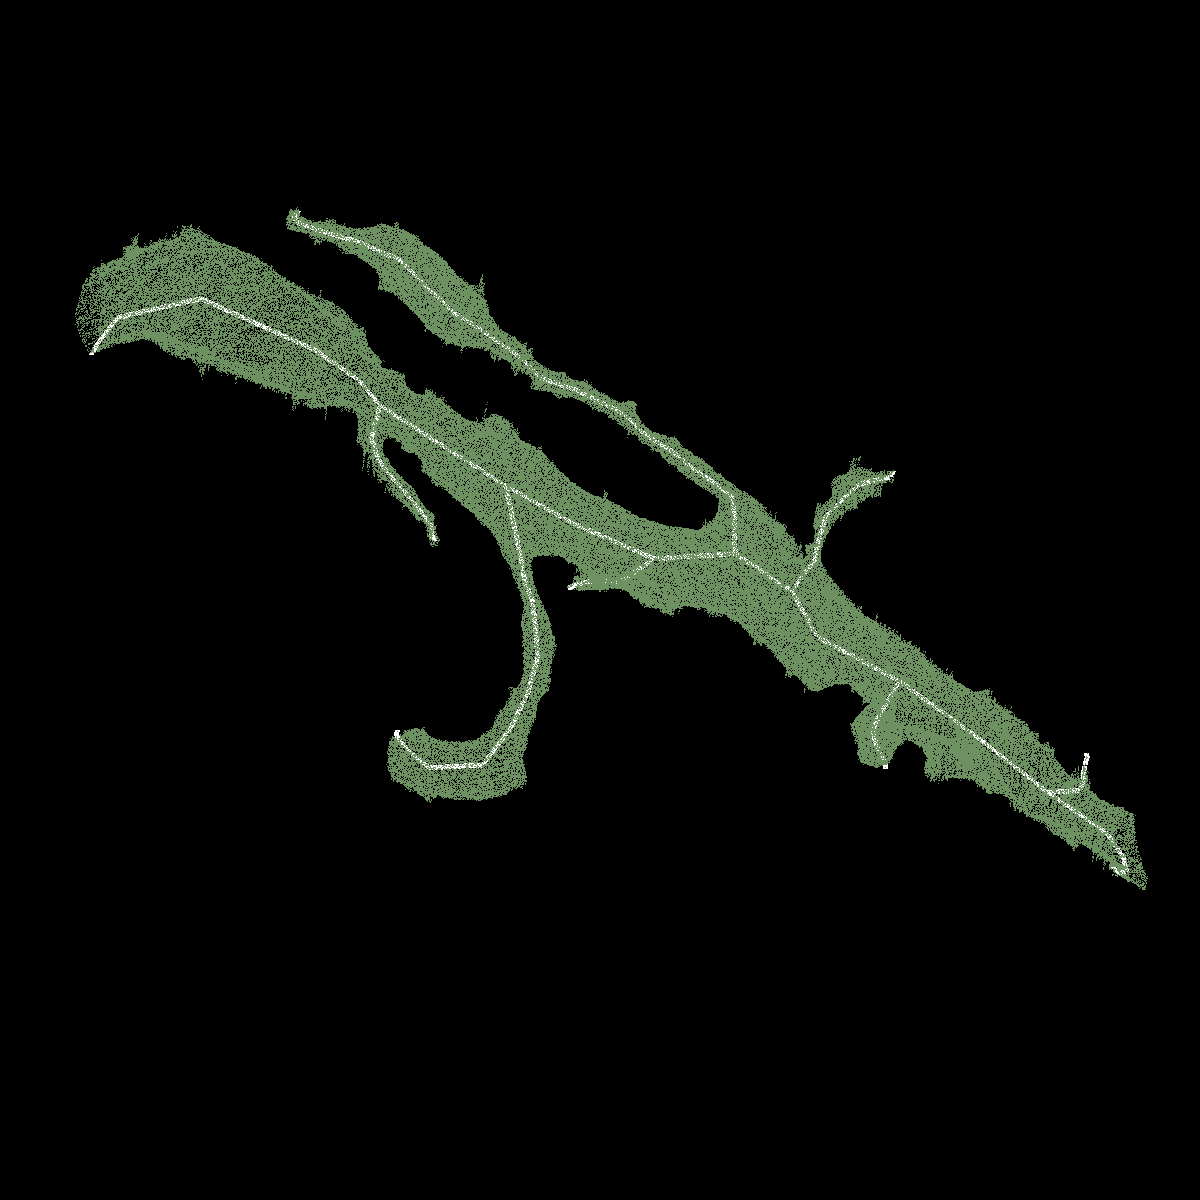
\includegraphics[width=0.42\linewidth]{./figures/skeleton2.png}
	\caption{Two example outputs of the TEASER skeletonization algorithm.}
	\label{fig:skeletonization}
\end{figure}

%\begin{algorithm}
	\begin{algorithmic}
		\Function{GenerateEdges}{$skeletons$}
			\For {$skeleton$ in $skeletons$}
				\State $candidates$ = set()
				\For {$endpoint$ in $skeleton$}
					
				\EndFor
			\EndFor
		\EndFunction
	\end{algorithmic}
%	\caption{Edge generation function}
%	\label{alg:generate-edges}
%\end{algorithm}

It is important to note that the above algorithm does not enforce neighboring voxel constraints on nearby segments. There are instances where two segments belong to the same neuron but the segments produced by the per-pixel and per-superpixel algorithms are non-adjacent. Figure (ADD FIGURE) shows two such examples that are not considered by previous research in this field. Finding and merge these examples is one of the benefits of retreating from per-pixel algorithms. Neither of these examples could merge under the GALA or NeuroProof pipelines.

\subsection{Edge Probabilities}

The previous section outlines how to generate edges between nodes in our graph structure. Here we will introduce a neural network architecture for generating probabilities that two nodes sharing an edge belong to the same neuron. The neural network takes as input only data from the input segmentation. 

\subsubsection{Network Architecture}

\begin{figure*}[t]
	\centering
	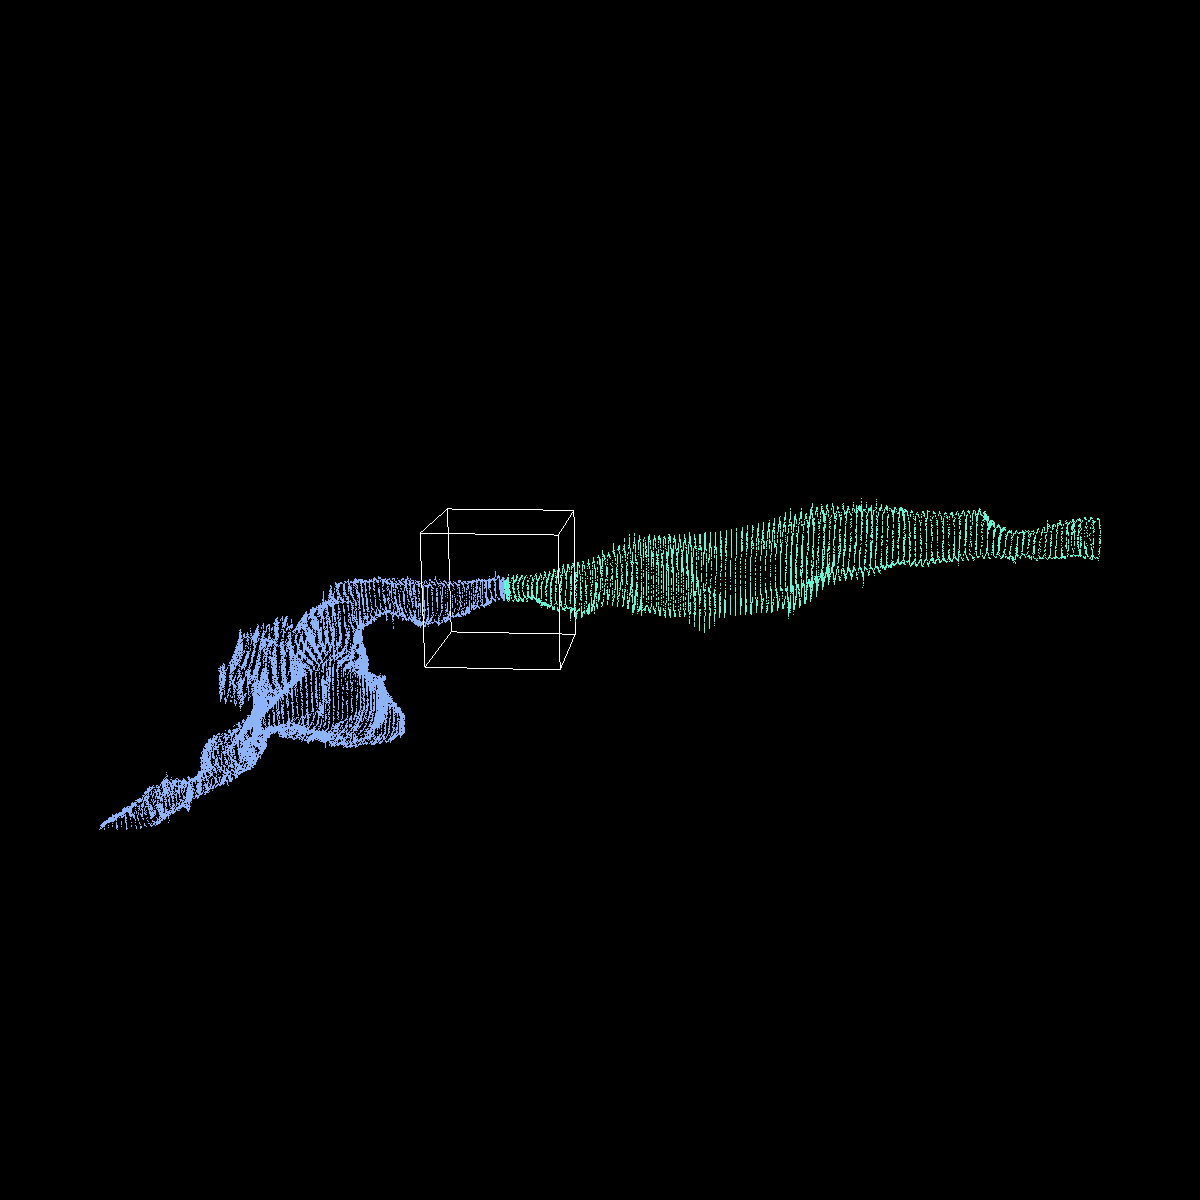
\includegraphics[width=0.3\linewidth]{./figures/network_distance_400.png}
	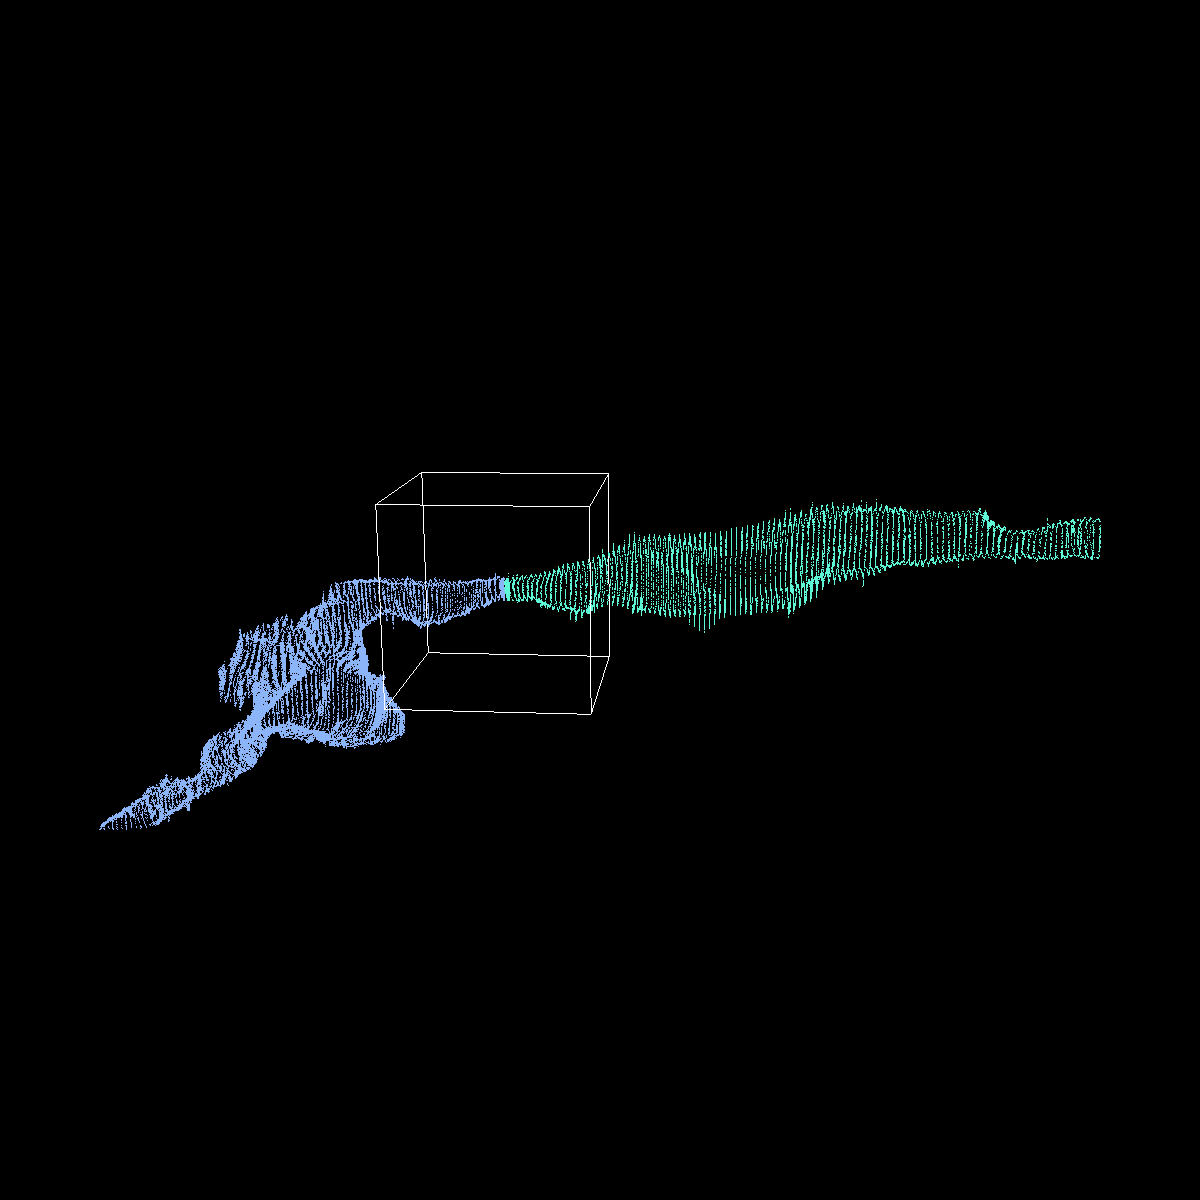
\includegraphics[width=0.3\linewidth]{./figures/network_distance_600.png}
	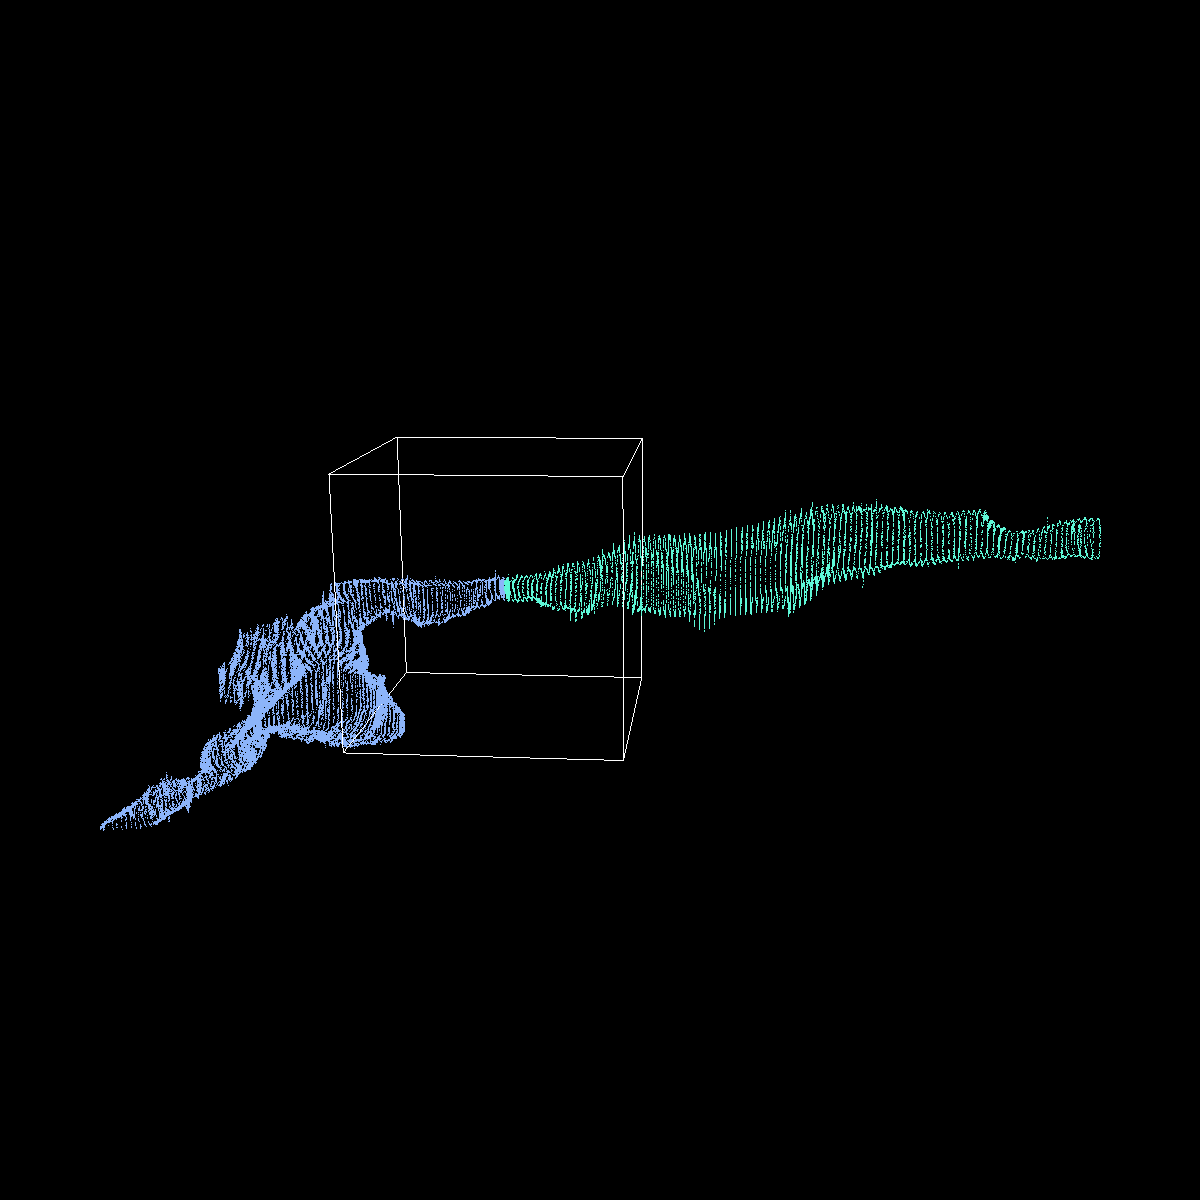
\includegraphics[width=0.3\linewidth]{./figures/network_distance_800.png}	
	\caption{The white outlines show three different possible cubic sizes to input into the neural network. The left example ($800\textrm{nm}$) provides less local context than the middle example ($1200\textrm{nm}$). The right example ($1600\textrm{nm}$) extracts too large of a local region that produces noise as one of the segments leaves the bounding box only to reenter.}
	\label{fig:network-radius}
\end{figure*}


The above skeletonization algorithm produces 3D locations that require further consideration for merging. To determine which of these segments should actually merge, we train a 3-D convolutional neural network. We extract a cubic region with length $1200\textrm{nm}$ centered at these locations. These cubes will provide the local information for the neural network to predict which neighboring segments belong to the same neuron. A cubic length of $1200\textrm{nm}$ provides enough local shape context for the network without introducing an excessive amount of noise. Figure \ref{fig:network-radius} shows cubes of lengths $800\textrm{nm}, 1200\textrm{nm},$ and $1600\textrm{nm}$.

We transform the extracted cubes for input into the neural network. The network takes three input channels for each voxel in the 3-D volume corresponding to the following mapping. Consider a pair of segments with labels $l_1$ and $l_2$ for every voxel $v$ in the cube of interest. The first channel is $0.5$ if $v = l_1$ and $-0.5$ otherwise, the second channel is $0.5$ if $v = l_2$ and $-0.5$ otherwise, and the third channel is $0.5$ if $v = l_1$ or $v = l_2$ and $-0.5$ otherwise. 

Each 3-channel volume is subsequently downsampled into an array of size $(3, 22, 68, 68)$ using nearest-neighbor interpolation. Our neural network trains on these 4-D arrays to generate probabilities that $l_1$ and $l_2$ should merge for every input.

Our network architecture has three layers of double convolutions followed by a max pooling step \cite{chatfield2014return}. As described above, the input with into the network is $(22, 68, 68)$ with $3$ channels. The filter size of the layers are 16, 32, and 64 with size doubling deeper into the network. The first two max pooling layers are anisotropic with pooling only in $x$ and $y$ to match the anisotropic nature of our EM datasets. All convolutions have kernel sizes of $(3, 3, 3)$. The output size of the final max pooling layer is $(5, 5, 5)$ with $64$ channels. The output is flattened into a 1-D vector with $8000$ entries which enters two fully connected layers with $512$ and $1$ dimensions in the output respectively. All activation functions are LeakyReLU with $\alpha=0.001$ except for the final activation which uses a sigmoid function \cite{funahashi1989approximate,maas2013rectifier}. There is a dropout of $0.2$ after every pooling layer and the first dense layer. There is a dropout of $0.5$ after the final dense layer. The above method uses stochastic gradient descent with Nesterov's Accelerated Gradient \cite{nesterov1983method}. This optimizer has an initial learning rate of $0.01$, momentum of $0.9$, and a decay rate of $5*10^{-8}$. Figure \ref{fig:architecture} provides an overview of the proposed architecture. 

\begin{figure*}[t]
	\centering
	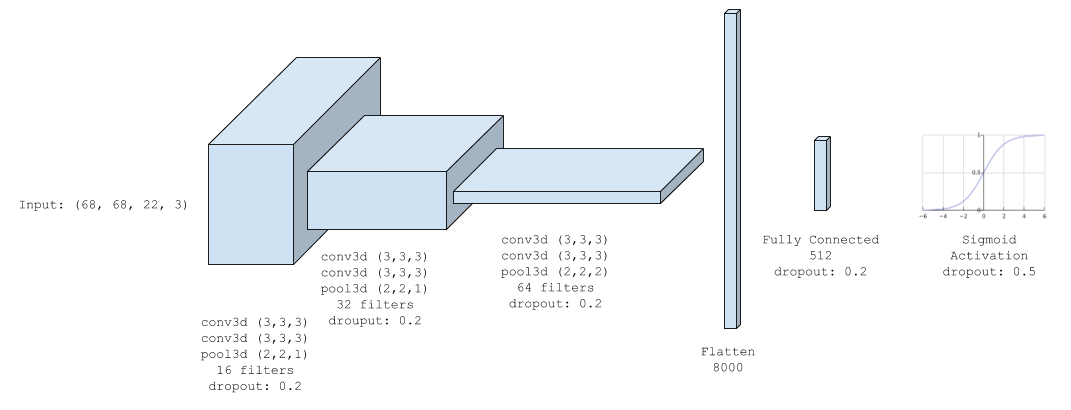
\includegraphics[width=0.95\linewidth]{figures/architecture.png}
	\caption{The architecture for the neural networks follows the \textit{VGG} style of double convolutions followed by a max pooling operation. The number of filters doubles each layer leading to a fully connected layer and a sigmoid activation function.}
	\label{fig:architecture}
\end{figure*}


\subsubsection{Data Augmentation}

Manual labeling of connectomics datasets is time intensive and expensive (CITE?). As we consider higher levels of abstractions of the data, the amount of useful labeled data decreases. This follows from the simple fact that manual annotation of the data happens at the per-pixel level, so starting with larger agglomerated segments leads to fewer unique human labels (THIS DOESN'T MAKE SENSE YET). 

Therefore, we apply some data augmentation to the generated examples to increase the size of the training datasets. We consider all rotations of $90$ degrees along the $xy$-plane in addition to mirrors along the $x$ and $z$ axes. This produces an additional 16 times more training data. 

\subsection{Agglomeration}

After constructing the above graph structure we can apply a graph-based segmentation strategy. There are many formulations of graph-based optimization strategies that provide different guarantees on their output. Neurons in the brain should be acyclic, i.e. the output shape should have a genus of zero. Current connectomics agglomeration techniques do not leverage this additional information but rather consider neighboring regions in successive order without regard to created loops. In our graph formulation we can enforce this topological property by applying a multicut partition onto the graph which generates a forest on the nodes. There are several heuristics that solve the multicut problem. For our purposes we use the Kernighan-Lin algorithm \cite{kernighan1970efficient}.